\ifdefined\included
\else
\documentclass[french, a4paper, 11pt, twoside, pdftex]{StyleThese}
\usepackage{iflang}
\usepackage{bibentry}



%\usepackage[sectionbib]{chapterbib}          % Cross-reference package (Natural BiB)
%\usepackage{natbib}                  % Put References at the end of each chapter
%\usepackage{bibunits}
% Do not put 'sectionbib' option here.
% Sectionbib option in 'natbib' will do.


\usepackage{fancyhdr}                    % Fancy Header and Footer

\usepackage[utf8]{inputenc}
\usepackage[T1]{fontenc}
\usepackage[french]{babel} %
\usepackage{lmodern} \normalfont %to load T1lmr.fd 
\DeclareFontShape{T1}{cmr}{b}{sc} { <-> ssub * cmr/bx/sc }{}
%\hyphenation{gar}

\usepackage{amsmath,amssymb}             % AMS Math
\usepackage{nicefrac}
\usepackage{siunitx}					%% Unites Math SI

\usepackage{blindtext}

\usepackage{datetime}

\usepackage{lipsum} 

\usepackage[inline]{enumitem}

\usepackage{hhline}
%\usepackage[left=1.5in,right=1.3in,top=1.1in,bottom=1.1in]{geometry}
\usepackage[left=1.5in,right=1.3in,top=1.1in,bottom=1.1in,includefoot,includehead,headheight=13.6pt]{geometry}

%%\renewcommand{\baselinestretch}{1.05}

%%%%%%%% Multi-figures avec sub-captions
\usepackage{caption}
\usepackage{subcaption}

% Table of contents for each chapter

\usepackage[nottoc, notlof, notlot]{tocbibind}
\usepackage[nohints]{minitoc}
\setcounter{minitocdepth}{2}
\mtcindent=15pt
% Use \minitoc where to put a table of contents

\usepackage{aecompl}

%% Package cosmetic meilleur layout du texte en jouant sur le spacing par caractères
\usepackage[activate={true,nocompatibility},final,tracking=true,kerning=true,factor=1100,stretch=10,shrink=10]{microtype}
\usepackage[absolute,overlay]{textpos} 
\setlength{\TPHorizModule}{\paperwidth}\setlength{\TPVertModule}{\paperheight}
\sloppy

%%%%%%%%%%% JOLIS TABLEAUX
\usepackage{tabularx}		%\usepackage{tabular}
\usepackage{longtable}
\usepackage{multirow}
\newcommand{\mc}{\multicolumn} 
\newcommand{\mr}[2]{\multirow{#1}{*}{#2}} 	\newcommand{\mrQ}{\multirow{-4}{*}}
\usepackage{booktabs}

\usepackage[usenames,dvipsnames]{xcolor} 

\makeatletter
\newcommand{\ccolor}[3][]{%
	\kern-\fboxsep
	\if\relax\detokenize{#1}\relax
	\expandafter\@firstoftwo
	\else
	\expandafter\@secondoftwo
	\fi
	{\colorbox{#2}}%
	{\colorbox[#1]{#2}}%
	{#3}\kern-\fboxsep
}
\makeatother

%%%%% Insertion graphiques format PGF
\usepackage{pgfplots}
\pgfplotsset{width=\linewidth, compat=1.16}%, compat=1.17}
\usepackage{adjustbox}          %%% PERMET DE LES RECADRER + FACILEMENT


%%%%%%%%%% Bullets de listes sans saut de ligne %%%%%%%%%%
\usepackage{xparse}

\ExplSyntaxOn%
\seq_new:N \l_local_enum_seq

\newcommand{\storethestuff}[1]{%
  \seq_set_from_clist:Nn \l_local_enum_seq {#1}%
}

\newcommand{\dotheenumstuff}{%
\int_zero:N \l_tmpa_int
\seq_map_inline:Nn \l_local_enum_seq {%
    \int_incr:N \l_tmpa_int% Increase the counter
    \item ##1
    % Check whether the list has reached the end -- if so, use '.' instead of ','
    %\int_compare:nNnTF 
    % { \l_tmpa_int } < {\seq_count:N \l_local_enum_seq} 
    % {,} {.}
  }
}
\ExplSyntaxOff

\NewDocumentCommand{\linebullets}{+m}{%
  \storethestuff{#1}%
  \begin{enumerate*}[label={\alph*)},font={\bfseries},itemjoin={{, }}]
    \dotheenumstuff%
  \end{enumerate*}
}

\newcommand{\cmnt}[1]{}  %%%%% AJOUT DE COMMENTAIRE MULTILIGNES


%%%%%%%%%% ECRITURE CARACTERES DANS UN CERCLE %%%%%%%%%%
%\def\circleTxt[#1]{\raisebox{.5pt}{\textcircled{\raisebox{-1pt}{#1}}}}
\newcommand{\ctxt}[1]{\raisebox{.5pt}{\textcircled{\raisebox{-1.2pt}{#1}}}}
% Glossary / list of abbreviations

\usepackage[intoc]{nomencl}
\IfLanguageName{english}{%
\renewcommand{\nomname}{Glossary}
}{ %
\renewcommand{\nomname}{Liste des Abréviations}
}

\makenomenclature

% My pdf code

\usepackage{ifpdf}

\ifpdf
  \usepackage[pdftex]{graphicx}
  \DeclareGraphicsExtensions{.pdf,PDF,.png,PNG,.jpg,JPG}
  \usepackage[pagebackref,hyperindex=true]{hyperref} %% use \autoref{} instead of Table~\ref{}.
  \usepackage{tikz}
  \usetikzlibrary{arrows,shapes,calc}
\else
  \usepackage{graphicx}
  \DeclareGraphicsExtensions{.ps,.eps}
  \usepackage[a4paper,dvipdfm,pagebackref,hyperindex=true]{hyperref}
\fi

\graphicspath{{.}{schemas/}{graphiques/}{tables/}}

%% nicer backref links. NOTE: The flag ThesisInEnglish is used to define the
% language in the back references. Read more about it in These.tex

\IfLanguageName{english}{
\renewcommand*{\backref}[1]{}
\renewcommand*{\backrefalt}[4]{%
\ifcase #1 %
(Not cited.)%
\or
(Cited in page~#2.)%
\else
(Cited in pages~#2.)%
\fi}
\renewcommand*{\backrefsep}{, }
\renewcommand*{\backreftwosep}{ and~}
\renewcommand*{\backreflastsep}{ and~}
}{
\renewcommand*{\backref}[1]{}
\renewcommand*{\backrefalt}[4]{%
\ifcase #1 %
(Non cité.)%
\or
(Cité en page~#2.)%
\else
(Cité en pages~#2.)%
\fi}
\renewcommand*{\backrefsep}{, }
\renewcommand*{\backreftwosep}{ et~}
\renewcommand*{\backreflastsep}{ et~}
}

% Links in pdf
\usepackage{color}
\definecolor{linkcol}{rgb}{0,0,0.4} 
\definecolor{citecol}{rgb}{0.5,0,0} 
\definecolor{linkcol}{rgb}{0,0,0} 
\definecolor{citecol}{rgb}{0,0,0}
% Change this to change the informations included in the pdf file

\hypersetup
{
bookmarksopen=true,
pdftitle="Prévention des fautes temporelles sur architectures multicœur pour les systèmes à criticité mixte",
pdfauthor="Daniel LOCHE", %auteur du document
pdfsubject="Thèse", %sujet du document
%pdftoolbar=false, %barre d'outils non visible
pdfmenubar=true, %barre de menu visible
pdfhighlight=/O, %effet d'un clic sur un lien hypertexte
colorlinks=true, %couleurs sur les liens hypertextes
pdfpagemode=UseNone, %aucun mode de page
%pdfpagelayout=DoublePage, %ouverture en simple page
pdffitwindow=true, %pages ouvertes entierement dans toute la fenetre
linkcolor=linkcol, %couleur des liens hypertextes internes
citecolor=citecol, %couleur des liens pour les citations
urlcolor=linkcol %couleur des liens pour les url
}

% definitions.
% -------------------

\setcounter{secnumdepth}{3}
\setcounter{tocdepth}{2}

% Some useful commands and shortcut for maths:  partial derivative and stuff

\newcommand{\pd}[2]{\frac{\partial #1}{\partial #2}}
\def\abs{\operatorname{abs}}
\def\argmax{\operatornamewithlimits{arg\,max}}
\def\argmin{\operatornamewithlimits{arg\,min}}
\def\diag{\operatorname{Diag}}
\newcommand{\eqRef}[1]{(\ref{#1})}
\newcommand{\nline}{\smallbreak\noindent}

\usepackage{rotating}                    % Sideways of figures & tables

% \usepackage{txfonts}                     % Public Times New Roman text & math font
  
%%% Fancy Header %%%%%%%%%%%%%%%%%%%%%%%%%%%%%%%%%%%%%%%%%%%%%%%%%%%%%%%%%%%%%%%%%%
% Fancy Header Style Options

\pagestyle{fancy}                       % Sets fancy header and footer
\fancyfoot{}                            % Delete current footer settings

%\renewcommand{\chaptermark}[1]{         % Lower Case Chapter marker style
%  \markboth{\chaptername\ \thechapter.\ #1}}{}} %

%\renewcommand{\sectionmark}[1]{         % Lower case Section marker style
%  \markright{\thesection.\ #1}}         %

\fancyhead[LE,RO]{\bfseries\thepage}    % Page number (boldface) in left on even
% pages and right on odd pages
\fancyhead[RE]{\bfseries\nouppercase{\leftmark}}      % Chapter in the right on even pages
\fancyhead[LO]{\bfseries\nouppercase{\rightmark}}     % Section in the left on odd pages

\let\headruleORIG\headrule
\renewcommand{\headrule}{\color{black} \headruleORIG}
\renewcommand{\headrulewidth}{1.0pt}
\usepackage{colortbl}
\arrayrulecolor{black}

\fancypagestyle{plain}{
  \fancyhead{}
  \fancyfoot{}
  \renewcommand{\headrulewidth}{0pt} %%%%%%%%%%%%%%%%%%%%%%%%%%%%%%%%%%%%%%%%%%%%%%%%%%%%%%%%%%%%%%%%%%%%%%%%%%%%%%%%%%%%%
}

%\usepackage{MyAlgorithm}
%\usepackage[noend]{MyAlgorithmic}
%\usepackage[ED=EDSYS-SystEmb, Ets=INP]{tlsflyleaf}

%%% Clear Header %%%%%%%%%%%%%%%%%%%%%%%%%%%%%%%%%%%%%%%%%%%%%%%%%%%%%%%%%%%%%%%%%%
% Clear Header Style on the Last Empty Odd pages
\makeatletter

\def\cleardoublepage{\clearpage\if@twoside \ifodd\c@page\else%
  \hbox{}%
  \thispagestyle{empty}%              % Empty header styles
  \newpage%
  \if@twocolumn\hbox{}\newpage\fi\fi\fi}

\makeatother
 
%%%%%%%%%%%%%%%%%%%%%%%%%%%%%%%%%%%%%%%%%%%%%%%%%%%%%%%%%%%%%%%%%%%%%%%%%%%%%%% 
% Prints your review date and 'Draft Version' (From Josullvn, CS, CMU)
\newcommand{\reviewtimetoday}[2]{\special{!userdict begin
    /bop-hook{gsave 20 710 translate 45 rotate 0.8 setgray
      /Times-Roman findfont 12 scalefont setfont 0 0   moveto (#1) show
      0 -12 moveto (#2) show grestore}def end}}
% You can turn on or off this option.
% \reviewtimetoday{\today}{Draft Version}
%%%%%%%%%%%%%%%%%%%%%%%%%%%%%%%%%%%%%%%%%%%%%%%%%%%%%%%%%%%%%%%%%%%%%%%%%%%%%%% 

\newenvironment{maxime}[1]
{
	\def\Arg{#1}
\vspace*{0cm}
\hfill
\begin{minipage}{0.6\textwidth}%
%\rule[0.5ex]{\textwidth}{0.1mm}\\%
\hrulefill $\:$ \\%$\:$ {\bf #1}\\
%\vspace*{-0.25cm}
\it 
}%
{%
	
\hrulefill $\:$ {\bf \Arg}
\vspace*{0.5cm}%
\end{minipage}
}

\let\minitocORIG\minitoc
\renewcommand{\minitoc}{\minitocORIG \vspace{1.5em}}

%\usepackage{slashbox}

\newenvironment{bulletList}%
{ \begin{list}%
	{$\bullet$}%
	{\setlength{\labelwidth}{25pt}%
	 \setlength{\leftmargin}{30pt}%
	 \setlength{\itemsep}{\parsep}}}%
{ \end{list} }


%%%%%%% Outils pour \comment \alert \add %%%%%
\usepackage{easyReview}
\usepackage{soulutf8} % for accented letters

\let\newalert\alert
\renewcommand{\alert}[1]{\textit{\newalert{#1}}}

%\usepackage[commandnameprefix=ifneeded]{changes} %% \chhighlight and \chcomment to avoid collision with easyReview
\renewcommand{\epsilon}{\varepsilon}

% centered page environment

\newenvironment{vcenterpage}
{\newpage\vspace*{\fill}\thispagestyle{empty}\renewcommand{\headrulewidth}{0pt}}
{\vspace*{\fill}}

\usepackage{tablefootnote}

%%%%%% MISE EN FORME CADRES DEFINITIONS/THEOREMES/LEMES %%%%%%%%%%
\usepackage{amsthm}  % for theoremstyle

\theoremstyle{plain} 
\newtheorem{theorem}{Théorème}[section]
\newtheorem{corollary}{Corolaire}[theorem]

%\theoremstyle{lemma}
%\newtheorem{lemma}[theorem]{Lemme}


\theoremstyle{definition}
\newtheorem{definition}[theorem]{Définition}


\cmnt{
	\usepackage{ntheorem} %\usepackage{amsthm}  % for theoremstyle
	%\usepackage{mdframed}
	\usepackage[most]{tcolorbox}
	
	\theoremstyle{plain} 
	\theoremindent20pt
	\theoremheaderfont{\normalfont\bfseries\hspace{-\theoremindent}}
	\newtheorem{theorem}{Théorème}[section]
	\newtheorem{corollary}{Corolaire}[theorem]
	
	\theoremstyle{plain}
	\newtheorem{lemma}[theorem]{Lemme}
	
	
	\tcolorboxenvironment{theorem}{
		blanker,
		breakable,
		before skip=\topsep,
		after skip=\topsep,
		borderline west={1pt}{10pt}{double, shorten <=12pt}
	}
	
	\theorembodyfont{\normalfont}
	\theoremindent20pt
	\theoremheaderfont{\normalfont\bfseries\hspace{-\theoremindent}}
	\newtheorem{definition}[theorem]{Définition}
	
	
	\tcolorboxenvironment{definition}{
		blanker,
		breakable,
		before skip=\topsep,
		after skip=\topsep,
		borderline west={1pt}{10pt}{shorten <=12pt}
	}
}

\cmnt{ 
	\begin{theorem}
		Ceci est un Théorème.
	\end{theorem} 
	
	\begin{corollary}
		Ceci est un Corollaire.
	\end{corollary}
	
	\begin{definition}
		Ceci est une Définition.
	\end{definition}
	
	\begin{lemma}
		Ceci est un Lemme.
	\end{lemma}
}

\def\UrlBigBreaks{\do\/\do-\do:}
\usepackage{url}

\DeclareUnicodeCharacter{202F}{\,}
\sloppy

\begin{document}
\setcounter{chapter}{1}
\dominitoc
\faketableofcontents
\fi

\chapter{Contexte et Enjeux des Systèmes Embarqués} \label{chap:1_EnjeuxIntro}
\minitoc

La conception des systèmes embarqués, typiquement automobiles, a subi de fortes évolutions orientées vers de nouvelles fonctionnalités centrées sur le logiciel. 
Ces évolutions demandent des capacités de calcul de plus en plus importantes et donc des architectures matérielles pour supporter la demande grandissante en fonctionnalités. 
Par ailleurs le contexte industriel mène à la disparition des calculateurs d'antan, monocœurs, pour se focaliser sur des calculateurs plus complexes et puissants, multicœurs. 
Cette tendance au multicœur provient à la fois d'une limitation technologique et d'un besoin grandissant~: la façon d'augmenter les capacités de calculs par les méthodes classiques (montée en fréquence) atteint ses limites et les capacités d'exécution concourante de logiciel est de plus en plus demandée dans un contexte aux contraintes financières et de \textit{time-to-market} fortes. 
C'est ainsi que né la volonté de passer sur des architectures électriques et électroniques plus centralisées via l'utilisation d'une quantité réduite d'unités de calcul, mais intégrant un plus grand nombre de fonctionnalités de traitement en leur sein ; en un mot, des processeurs multicœurs. Cette volonté implique cependant une superposition des difficultés inhérentes aux architectures matérielles plus complexes avec les contraintes de sûreté de fonctionnement du logiciel. Nous faisons donc face à des systèmes à criticité mixte exécutés sur des calculateurs aux mécanismes complexes. Nous verrons ainsi dans ce chapitre quels sont les aspects essentiels de ce contexte et ses spécificités à prendre en compte pour proposer de nouveaux éléments de réponse dans la conception de systèmes à criticité mixte sur processeurs multicœurs. Nous conclurons cette partie avec la présentation de la problématique à laquelle nous tenterons de répondre ainsi que la présentation des différents chapitres de cette thèse.

\section{Évolutions des Systèmes embarqués}
	\subsection{Nouveaux systèmes intelligents et connectés}
		Si l'on prend le cas du domaine automobile, depuis près de trente ans l'industrie n'a cessé de faire évoluer la façon de concevoir les véhicules et notamment leurs systèmes sous-jacents. Comme illustré avec le  diagramme~\ref{fig:evo_sys_automobile}, la transition s'est faite de modifications purement mécaniques vers des évolutions électriques, puis électroniques et de plus en plus intelligentes. Les systèmes de divertissement du consommateur ont été les premiers, dans le milieu des années 1920, à introduire des composants électroniques au sein des véhicules sous la forme de récepteurs radio à lampes ! Si l’apparition de transistors, dans les années 1950, a contribué à	l’amélioration des capacités techniques des appareils et à la diffusion massive des autoradios au sein des automobiles, le concept de base a peu évolué jusqu'à la fin des années 1970. L’introduction des premiers systèmes de navigation dans les années 1980, puis des systèmes multimédia dans les années 2000 a changé la donne. Désormais, l'ancienne façade de l’autoradio devient un écran de commande nommée \emph{head unit} et concentre 70\% du code du véhicule.	Les voitures se sont modernisées avec l'ajout de calculateurs dédiés à des fonctions internes ou des services. Le développement des technologies de l'industrie {4.0} mène à une augmentation exponentielle du logiciel embarqué dans l'automobile au cours des 15 dernières années~\cite{blanchet_industrie_2016}, avec la présence de plus de 60 calculateurs embarqués dans certains modèles. Les contrôles mécaniques et autres systèmes électriques "simples" cèdent la place au monde du numérique. Les équipements électroniques et logiciels se multiplient au sein du véhicule pour l’aide à la conduite (\textit{Advanced Driver-Assistance System -- ADAS}) et l’ajout de services~\cite{schmidt_automotive_2010}. De fait, le système multimédia moderne a un rôle qui va bien au-delà de celui du simple autoradio~: il devient l'interaction principale entre le consommateur et le véhicule et devient un critère de choix prépondérant à l'achat.
		
		% le nombre de fonctionnalité d'aide à la conduite a explosé. 
		\begin{figure}[ht]
			\centering
			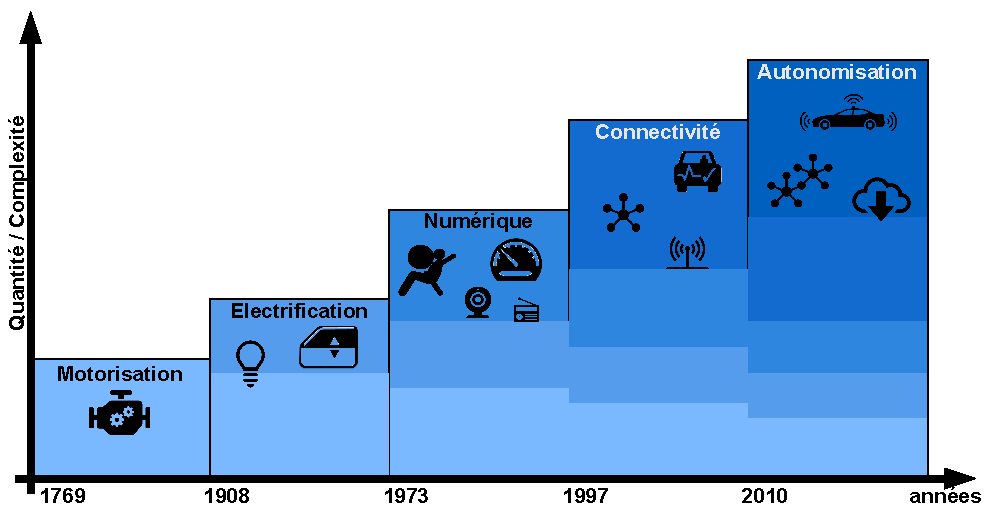
\includegraphics[width=0.9\linewidth]{schemas/Evo_Sys_Automobile}
			\caption[Évolutions des Systèmes Automobiles]{Principaux domaines d'évolution des systèmes automobiles au fil du temps}
			\label{fig:evo_sys_automobile}
		\end{figure}

		Ainsi, du simple Système Anti-blocage des roues (ABS), on a introduit des Assistants à la Conduite tels que le Freinage d'Urgence (\textit{Emergency Braking System}) ou encore le Système de Gestion de Ligne (\textit{Lane Support System}) qui permet à la fois l'Avertissement de Dépassement de Ligne (\textit{Lane Departure Warning}), l'Assistant de Maintien de Ligne (\textit{Lane Keeping Assist}) et le Maintien de Ligne d'Urgence (\textit{Emergency Lane Keeping})... et il ne s'agit là que de 2 fonctionnalités supplémentaires~! En parallèle, la voiture devient de plus en plus automatisée, voire autonome. Elle gagne en connectivité avec la prise en compte de données extérieures possiblement avec un lien direct au cloud pour proposer une diversité de services~: météo, divertissement, trafic routier, pour n'en citer que quelques exemples.
		Les systèmes embarqués deviennent par conséquent aussi connectés. On parle de communications \emph{car-to-car} entre véhicules ou \emph{car-to-infrastructure} entre véhicule et infrastructures routières par exemple. 
		Cette ouverture du système à son environnement est à double tranchant. D'une part cela offre de nouveaux horizons de fonctionnalités et optimisations de conduite, avec des possibilités d'évolutivité simplifiée. Mais d'autre part la complexité va grandissante avec les enjeux d'ingénierie que cela implique. %%%check si bon endroit pour ça
		 
		%%%%%%%%% Emergence des architectures EE actuelles GENERALISATION 
		De façon plus générale, le contexte industriel actuel fait émerger de nouvelles technologies basées sur des logiciels de plus en plus complexes et performants. Cela est rendu possible via l'émergence d'architectures matérielles toujours plus puissantes et performantes. Ces améliorations permettent le développement et la mise en application de nouvelles technologies comme les réseaux de communication sans fil haute performance ou encore l'usage d'intelligences artificielles. On retrouve ainsi un nombre grandissant de fonctionnalités directement embarquées dans l'automobile, l'avion, le train pour répondre à la fois à de nouveaux besoins fonctionnels~: assistance à la conduite/pilotage, tableaux de bord, etc. et à des besoins de confort d'usage~: info-divertissement, connectivité, automatisations... 
		
		
		D'un point de vue logiciel, les mises à jour de systèmes embarqués incluent à la fois de nouvelles fonctionnalités critiques pour le bon fonctionnement du système, mais aussi l'ajouts de fonctions moins critiques. Ces mises à jour de services non essentiels amplifient  la multiplicité des niveaux de criticités du logiciel embarqué et donc la cohabitation entre sous-systèmes critiques et sous-systèmes non-critiques que l'on pourrait qualifier de "confort". 
		
		\begin{figure}[ht]
			\centering
			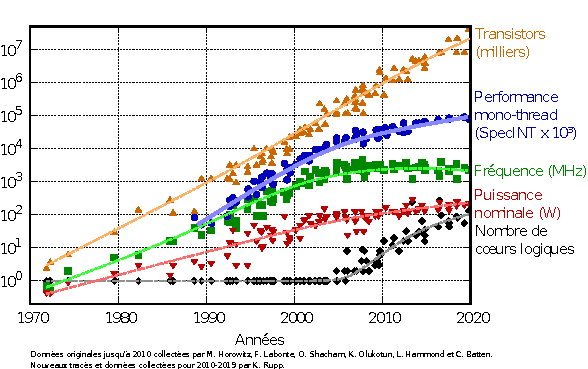
\includegraphics[width=0.8\linewidth]{graphiques/processors_trend}
			\caption[Évolution des processeurs]{42 Ans d'évolution des processeurs - Tendances}
			\label{fig:processorstrend}
		\end{figure}
		
		
		D'un point de vue matériel, il y a de fortes convergences sur les architectures employées dans les différents domaines. Historiquement, on retrouvait en premier lieu des calculateurs monocœurs. Cependant, les diverses évolutions d'exigences ont fait apparaître des limites en capacité de calcul. La montée en fréquence de fonctionnement atteint un seuil maximum à cause de la chauffe et la consommation que cela implique. Tandis que l'augmentation du nombre de transistors qui composent les processeurs arrive aux abords des limites physiques~: la taille de gravure du silicium arrive au même ordre de grandeur que la taille des atomes de silicium dont elle est composé. De fait, jusqu'à récemment encore, la Loi de Moore~\cite{thompson_moores_2006} sur la puissance des processeurs s'est vérifiée. Des premiers microprocesseurs Intel en 1971, avec quelques milliers de transistors de \SI{10}{\micro\metre}, l'on est aujourd'hui à plus de 1 milliards de transistors de près de \SI{10}{\nano\metre}. Mais à l'aune d'une gravure proche des \SI{2}{\nano\metre}, on environne les dimensions de 10 à 15 atomes et les effets de la physique quantique entrent en jeux. Par conséquent, l'on se dirige vers les limites des technologies actuelles pour poursuivre ces améliorations de puissance. Pour ces raisons, le plus grand levier de progression disponible aujourd'hui repose sur la parallélisation des unités de calcul, et donc la notion de calculateur multicœur, qui est apparue dès les années 1950~\cite{smotherman2005history}. Les fondeurs s'orientent vers des processeurs où la montée en puissance est assurée par la multiplication des unités de calcul (dit "cœurs") parallèles dans le processeur. On passe ainsi de monocœurs toujours plus petits et compacts à des duals/quadri cœurs... et l'on va aujourd'hui jusqu'à des supercalculateurs à plus de 128 cœurs. Tous ces changements se visualisent parfaitement avec l'évolution des caractéristiques des processeurs au fil des années en~\, tel qu'agrégé par K. Rupp~\cite{rupp_42_2020}. Cette évolution est la bienvenue dans tous les secteurs concernés, allant du grand public dans les ordinateurs, téléphones et autres multimédias jusqu'aux applications industrielles en passant par les usages de serveurs réseaux et centres de calculs.
		
		%%%%%%%% ARCHITECTURES MATERIELLES %%%%%%
		Il existe divers types d'architectures matérielles parmi les évolutions multicœurs que l'on retrouve aujourd'hui. On pourrait de façon simple différencier entre les multicœurs classiques, les manycœurs et à l'extrême ce que l'on connaît sous le nom de GPU, les processeurs graphiques.
		
		\paragraph{Multicœurs "classiques"}
			Les calculateurs multicœurs "classiques" disposent d'un certain nombre d'unités de calculs ("cœurs"), auxquelles sont adjointes diverses zones mémoires (cache, RAM, ROM). Le tout est piloté par des contrôleurs et bus de transferts de données pour interconnecter les cœurs, les cellules mémoires et les entrées/sorties. Dans les versions les plus récentes, des modules dédiés peuvent être ajoutés pour des fonctionnalités spécifiques comme le chiffrement. 
			
			La mémoire est partagée à différents degrés entre les cœurs. De façon à décongestionner les accès mémoire et accélérer ces dernières, une hiérarchie mémoire est mise en place, associant des espaces mémoire progressivement plus petits et rapides en fonction de leur proximité au processeur. Il s'agit ici de trouver un équilibre entre coût de la mémoire et vitesse d'accès aux données. En effet,  cette dernière dispose de trois caractéristiques antagonistes~: 
					\begin{itemize}
							\item la \textbf{latence} - temps d'accès aux données, 
							\item la \textbf{bande passante} - débit de données accessible,
							\item la \textbf{taille} mémoire - espace mémoire disponible (pour un coût donné).
						\end{itemize}
			Un espace mémoire pourra être soit de petite taille, mais rapide au niveau de son temps d'accès, soit de grande taille et plus lent comme schématisé dans la~\autoref{fig:hierarchiememoire}.  On a par conséquent au plus proche des cœurs les registres, de taille très limitée (octets) mais au temps d'accès très rapide~: ils sont la base pour toutes les opérations effectuées par le processeur. À l'opposé, la mémoire principale, de très grande taille (Go/To) pour laquelle tous les cœurs doivent passer par un bus commun pour y accéder. C'est donc la mémoire la plus lente d'accès mais aussi la moins coûteuse. Plusieurs intermédiaires ont été mis en place entre ces deux types de mémoire. Il s'agit typiquement de niveaux de cache qui peuvent être non partagés, c'est-à-dire propres à chaque cœur ou bien commun à tous. Le dernier niveau de cache, partagé, est classiquement appelé LLC (\emph{Last Level Cache}) et donne la limite entre les espaces mémoire limités en cache avec des accès rapides d'une part et la mémoire principale qui va provoquer de grands ralentissements d'autre part. 			
			On retrouve ainsi avec l'exemple de la~\autoref{fig:multicoeurintel} un cas de calculateur multicœur basé sur le cache, avec 8 cœurs, des niveaux de cache mémoire séparés (L1 et L2) et partagé (L3) ainsi que le bus d'accès à la mémoire principale. 
			
			%%%%% A DEPLACER DANS STRATEGIES EXISTANTES %%%%
			La gestion du contenu de ces caches (en lecture et écriture) est géré par une politique d'accès mémoire. Cette politique est essentielle à un usage efficace des caches du fait de leur espace limité qui demande à faire des choix sur son usage. Cela est peu documenté par les constructeurs,  et chacun aura sa façon de faire.
			La méthode de base la plus répandue étant empirique, par principe de localité temporelle~\cite{durrieu2014predictable} et spatiale~\cite{wilkes1965slave}. On considère que plus une donnée a été récemment accédée, plus elle a de chance d'être à nouveau utilisée. De même si une donnée est sollicitée, alors les données proches spatialement ont aussi plus de chance d'être utilisées. 
			Nous n'iront pas plus dans les détails sur les politiques de gestion d'accès à la mémoire. Il faut garder à l'esprit qu'elle est plutôt subie par les industriels qui intègrent le matériel dans leurs systèmes. Pour un processeur donné on aura certaines performances de calcul et accès mémoire, et il faudra mettre en comparaison les performances "par défaut" d'un logiciel sur une architecture donnée face au même système, \comment{pas clair ?}{mais avec des surcouches de gestion du logiciel apportées par l'intégrateur}.

			
			
\begin{figure}[ht]
	\centering
	\begin{subfigure}{.45\textwidth} \centering
		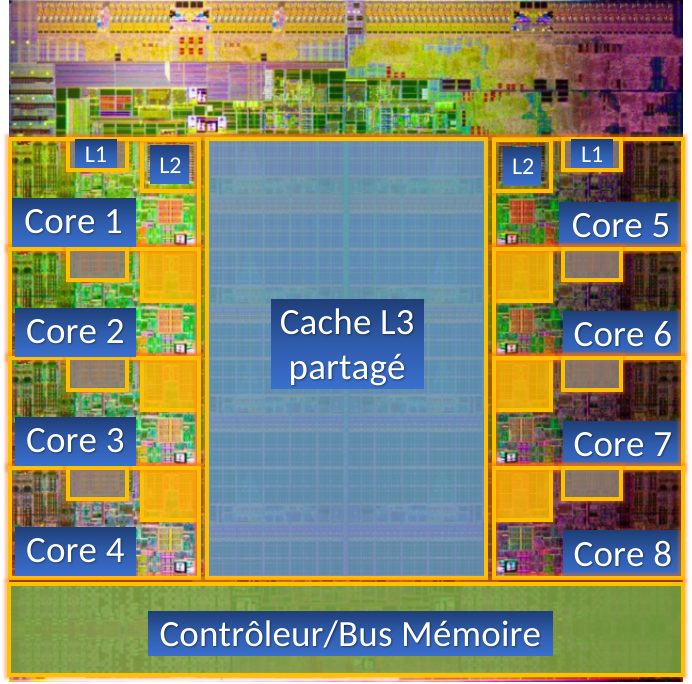
\includegraphics[width=0.9\linewidth]{schemas/multicoeurIntel}
		\caption{Exemple d'architecture multicœur}
		\label{fig:multicoeurintel}
	\end{subfigure}			
	\begin{subfigure}{.45\textwidth} \centering
		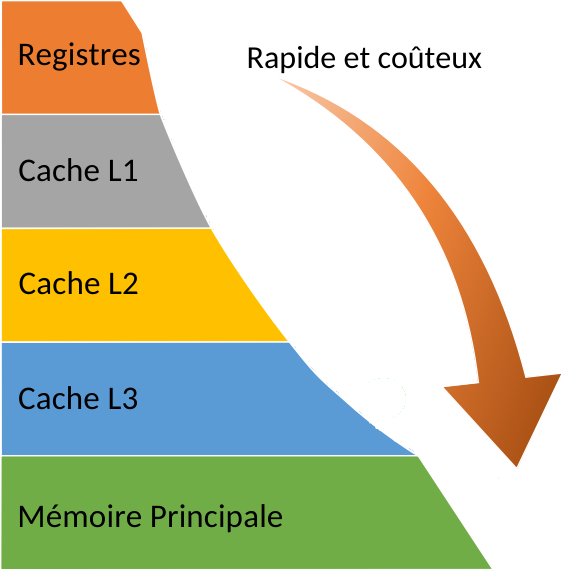
\includegraphics[width=0.85\linewidth]{schemas/hierarchieMemoire}
		\caption[Hiérarchie mémoire]{Schématisation de la hiérarchie mémoire selon leur coût et performance}
		\label{fig:hierarchiememoire}
	\end{subfigure}
	\caption{Exemple multicœur et mémoires}
	\label{fig:multicoeurs}
\end{figure}

			Il existe des variations d'architectures différentes selon les fondeurs, que l'on peut classifier en deux catégories principales. D'une part les multicœurs basés sur le cache (comme celui susmentionné) et d'autre part les multicœurs basés sur \emph{scratchpad}, c'est-à-dire des mémoires locales dédiées à chaque cœur. On peut voir la différence fondamentale de structure entre ces deux variations sur la~\autoref{fig:ArchitecturesMulticoeur}. 
			\comment{\textbf{TBA}}{Voir où et comment parler des multicœurs scratchpad ! Potentiellement dans "Solutions existantes".} 


\begin{figure}[ht]
	\centering
	\begin{subfigure}{.45\textwidth} \centering
		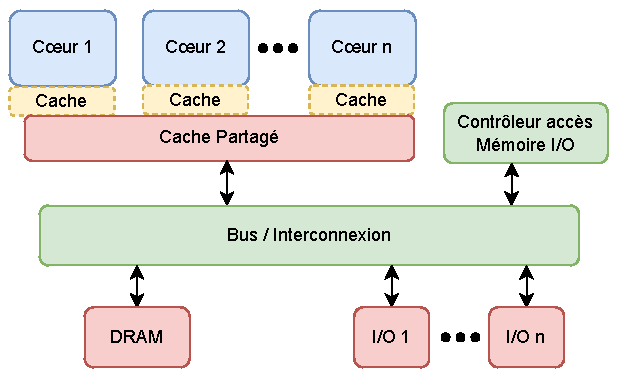
\includegraphics[width=\linewidth]{schemas/Multicore-CacheBased}
		\caption[Diagramme Multicœur Cache]{Architecture calculateur multicœur basé sur le cache}
		\label{fig:multicoeurCache}
	\end{subfigure}
	\begin{subfigure}{.45\textwidth} \centering
		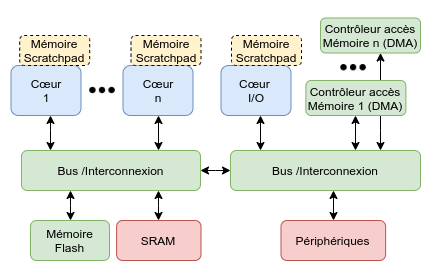
\includegraphics[width=\linewidth]{schemas/Multicore-ScratchpadBased}
		\caption[Diagramme Multicœur Scratchpad]{Architecture calculateur multicœur basé sur Scratchpad}
		\label{fig:multicœurScratchpad}
	\end{subfigure}
	\caption{Exemple multicœur et mémoires}
	\label{fig:ArchitecturesMulticoeur}
\end{figure}

		\paragraph{Calculateurs manycœurs}	Les calculateurs manycœurs sont des microprocesseurs incluant un grand nombre de cœurs dans l'objectif primaire d'une plus grande capacité d'exécution de code parallèle. Pour ce faire, les cœurs peuvent être spécialisés avec la réduction des instructions réalisables et optimisations à des tâches spécifiques. C'est la différence principale avec les multicœurs qui possèdent en en général des cœurs identiques (processeur homogène) avec de bonnes performances à la fois en série et en parallèle. 
		Les architectures manycœurs grâce à leurs spécificités demandent  des méthodes de programmation appropriées pour pouvoir être pleinement exploités dans le cadre d'une application. Cela augmente donc le niveau de complexité de développement, mais au bénéfice d'une forte amélioration des performances.
		
		Les GPUs (\emph{Graphic Processing Unit}) sont un cas particulier de manycœurs à présent très répandu pour des usages variés~\cite{owens2008gpu}. Cette forte expansion des GPU est due non seulement aux capacités de rendu graphique, mais surtout à leurs capacités de programmation parallèle poussée au maximum. Un grand nombre de domaines, notamment dans la recherche, y voient donc un microprocesseur d'usage général à hautes capacités de calcul parallèle.
		Les GPU sont efficaces du fait qu'ils permettent de réaliser le même calcul sur un très grand nombre de données différentes (typiquement calculs matriciels) pour obtenir tout autant de résultats en sortie. Il s'agit d'un modèle dit \emph{SIMD - Single-Instruction, Multiple-Data}. Là où les multicœurs conventionnels se focalisent sur des cœurs versatiles qui s'adaptent pour pouvoir gérer tous les cas d'applications, les GPU se focalisent sur la réalisation de tâches identiques en parallèles, ils restent donc spécialisés pour des types de tâches spécifiques, en complément de processeurs plus polyvalents.
		
		Dans le cadre de ces recherches, nous nous focaliseront sur le dénominateur commun le plus utilisé dans les architectures électriques et électroniques, qui est donc le processeur multicœur basé sur le cache.
		
\section{Risques et Problématique}
%%% Transition vers menaces
	Dans le cadre du contexte automobile, on se dirige \cmnt{de cette façon} vers un nouveau paradigme, où la voiture n'est plus un système mécanique sur lequel on adjoint du logiciel, mais à l'inverse un superordinateur multifonctionnel auquel on implante des roues et un moteur. 
	Les systèmes automobiles sont ainsi devenus des systèmes cyberphysiques qui entrent en interaction à la fois avec les utilisateurs et l'environnement. On distingue deux grands domaines de logiciels embarqués dans le véhicule. Tout d'abord l'info-divertissement, qui réunit les systèmes multimédias et autres affichages non nécessaires à l'usage primaire du véhicule. Et deuxièmement les calculateurs enfouis qui réalisent des fonctions essentielles qui ne sont pas nécessairement visibles de l'utilisateur, telles que le contrôle moteur. Pour soutenir ces besoins émergents, il est nécessaire de se baser sur des architectures matérielles plus puissantes comme les multicœurs. Cependant, cette disruption apporte de nouveaux enjeux, notamment de sécurité, vie privée, mais aussi sur la prédictibilité et la sûreté de fonctionnement du système à cause de sa complexification. Cela fait donc évoluer les systèmes embarqués dans un environnement profondément à risques, mais qui en plus s'accompagne de contraintes fortes. Nous nous devons donc d'introduire ici les notions de Sûreté de fonctionnement nécessaire à l'analyse.

	\subsection{Sûreté de Fonctionnement Informatique}~\label{sec:SureteDeFonctionnement}

		La sûreté de fonctionnement d’un système informatique (SdF) est "\textit{la propriété qui permet à ses utilisateurs de placer une confiance justifiée dans le service qu’il leur délivre, le service étant le comportement du système perçu par un utilisateur, cet utilisateur étant un système (informatique, humain, environnemental) qui interagit avec le premier.}"~\cite{arlat1995guide}. C’est donc la capacité d’un système informatique de répondre de manière correcte, conformément aux spécifications fonctionnelles, à une requête d’un autre système.  
		La sûreté de fonctionnement est définie en fonction de trois notions principales~: \linebullets{les \textit{attributs} qui définissent les propriétés assurées, les \textit{entraves} qui caractérisent les circonstances indésirables mais prévues, et les \textit{moyens} qui précisent les techniques permettant au système de fournir son service}.  
		Selon les services souhaités par l’utilisateur, ce dernier peut vouloir accentuer certaines propriétés pour assurer le bon fonctionnement du système. Ainsi la sûreté de fonctionnement englobe les attributs suivants~:  
		\begin{itemize}
			\item 	La \textbf{disponibilité} - la capacité d’être prêt à délivrer le service correct~; 
			\item 	La \textbf{fiabilité} - l’assurance de continuité d’un service correct~; 
			\item 	La \textbf{sécurité-innocuité} - l’assurance de non-propagation de conséquences catastrophiques à l’utilisateur ou l’environnement~; 
			\item 	L’\textbf{intégrité} - l’assurance de non-altération du système~; 
			\item 	La \textbf{maintenabilité} - l’aptitude à la réparation et à l’évolution du système. 
		\end{itemize} 
		Ces attributs permettent d’une part d’exprimer les propriétés devant être respectées par le système, et d’autre part d’évaluer la qualité du service délivré vis-à-vis de ces propriétés. Les aspects de sécurité, au sens de la confidentialité et des attaques face à des actions malveillantes indésirables ainsi que la confidentialité, c'est-à-dire, la non-divulgation d'information non autorisée, ne seront pas abordés dans cette thèse.
		
		Les entraves à la sûreté de fonctionnement sont les défaillances, les erreurs et les fautes. Une défaillance est une transition d’un service correct vers un service incorrect. Un service est considéré incorrect s’il n’est pas conforme à la spécification ou si la spécification ne décrit pas avec précision la fonction du système. Étant donné qu’un service consiste en une séquence d’états externes du système (observés par l’utilisateur), la survenue d’une défaillance signifie qu’au moins un des états externes s’écarte de l’état correct du service. La déviation est liée à une erreur, qui représente la partie de l’état interne du système pouvant entraîner une défaillance, dans le cas où elle atteint l’interface du service du système. La cause déterminée ou présumée d’une erreur est appelée une faute. La~\autoref{fig:suretedefonctionnemententraves} représente ce lien de cause à effet. Le fait de prévenir la causalité entre fautes est défaillances pour le bon fonctionnement se désigne par la méthode de silence sur défaillance. C'est-à-dire qu'une faute ou une erreur n'aura pas plus de conséquences et ne provoquera pas outre de défaillance, ou inversement.
		
		\begin{figure}[ht]
			\centering
			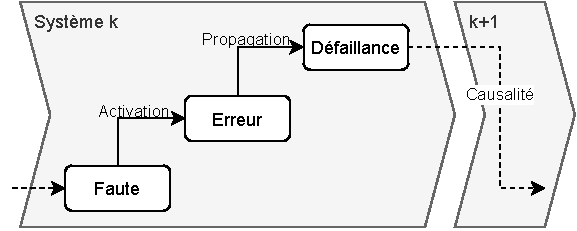
\includegraphics[width=0.7\linewidth]{schemas/SureteDeFonctionnement_entraves}
			\caption{Sûreté de fonctionnement - chaîne de causalité}
			\label{fig:suretedefonctionnemententraves}
		\end{figure}
		
		Pour minimiser l’impact de ces entraves, la sûreté de fonctionnement dispose de méthodes et techniques qui permettent de conforter les utilisateurs quant au bon accomplissement des fonctions du système. Le développement d’un système sûr de fonctionnement passe donc par l’utilisation combinée de ces méthodes, appelés moyens, pouvant être classées en quatre types~:
		\begin{itemize}
			\item \textbf{Prévision} des fautes~: estimation de la présence, de la création et des conséquences des fautes (p. ex. Analyse FMEA)~;
			\item \textbf{Prévention} des fautes~: méthodes visant à réduire les occurrences ou l’introduction de fautes (p. ex. outil de génie logiciel, processus de développement strict)~;
			\item \textbf{Élimination} des fautes~: réduction du nombre et de la sévérité des fautes (p. ex. test, injection de fautes)~;
			\item \textbf{Tolérance} aux fautes~: capacité de fournir un service, optimal ou dégradé, en présence de fautes (p. ex. techniques de redondance).
		\end{itemize}
	
		La prévention et la tolérance aux fautes visent à fournir la capacité de délivrer un service correct, tandis que l’élimination et la prévision des fautes visent à susciter la confiance en cette capacité en justifiant que les spécifications fonctionnelles de sûreté de fonctionnement et de sécurité sont adéquates et que le système est conforme. Toutes ces techniques sont dédiées à garantir des propriétés de sûreté de fonctionnement issues de spécification non fonctionnelles. % et non pas à délivrer un service applicatif.
		
		%%% PHRASE TRANSITION POURQUOI ON S'INTERESSE TaF
		%		Après avoir énoncé les principes fondamentaux de la sûreté de fonctionnement, nous allons nous intéresser plus précisément à la tolérance aux fautes.
		\paragraph{Tolérance aux Fautes}
		Les fautes auxquelles un système doit faire face sont nombreuses et peuvent ne pas avoir d’impact sur celui-ci tant qu’un ou plusieurs évènements ne se sont pas produits. On les appelle alors des fautes dormantes. Une fois activées, ces fautes peuvent avoir un impact catastrophique sur le système. D’origines diverses et variées, certaines fautes sont dues à l’environnement, au matériel, ou encore à l’être humain.
		
		Chaque faute peut provoquer une ou des erreurs différentes pouvant entraîner la défaillance du système. Malgré l’application des techniques de prévention et d’élimination des fautes, certaines subsistent et sont à même d’être activées.
		
		Un système tolérant aux fautes doit pouvoir assurer à l’utilisateur un service correct en dépit des fautes pouvant altérer ses composants, durant sa conception ou son interaction avec d’autres systèmes~\cite{avizienis_basic_2004}. La Tolérance aux fautes est mise en œuvre grâce aux moyens de \textbf{détection} d’erreurs, c.-à-d., l’identification des déviations du service correct, et de \textbf{recouvrement}, c.-à-d., les techniques permettant en cas d’erreur détectée de passer d’un état de système fautif à un état assurant un service nominal ou dégradé.
		
		La détection d’erreur peut être soit concurrente et se déroulant pendant l’exécution du système soit anticipée en vérifiant les paramètres du système lors de la suspension de son exécution. Une fois cette erreur détectée, les techniques de recouvrement peuvent être employées, d’une part pour assurer le service désiré et éviter la propagation de l’erreur (traitement des erreurs) et d’autre part pour isoler le composant fautif, diagnostiquer l’erreur, trouver et déterminer la faute originelle pour assurer une opération de maintenance (traitement des fautes).
		
		Les techniques de détection et de recouvrement sont nombreuses et sont regroupés dans des mécanismes de tolérance aux fautes associés à un ou plusieurs types de fautes. Il n’y a à l’heure actuelle aucun mécanisme générique pouvant pallier n’importe quel type de fautes ou d’erreurs. Que cela soit de la redondance matérielle, logicielle, temporelle, de la diversité dans l’implémentation ou l’architecture, les techniques sont nombreuses et souvent propres à chaque domaine et au budget alloué à la tolérance aux fautes.
		
		Dans le cadre de ces travaux de recherche, nous nous intéresseront particulièrement à la tolérance aux fautes qui attrait donc à la bonne exécution de tâches hébergées au sein d'un même calculateur. Dans le contexte industriel susmentionné, un même calculateur exécute des tâches pour des fonctionnalités variées et par conséquent avec des niveaux de criticité variés. Cela engendre notamment des contraintes sur les temps d'exécution des logiciels les plus critiques. C'est ce qu'on qualifie de systèmes temps réel. Nous sommes en résumé dans un contexte à criticité mixte, où du logiciel de système temps-réel va coexister avec du logiciel avec des contraintes temporelles moins strictes, voire aucune contrainte. L'implémentation de mécanismes de sûreté de fonctionnement dans ce contexte-là relève alors de la gestion de fautes temporelles dans un système à criticité mixte. 
		
\subsection{Systèmes temps-réel et Ressources partagées}
	\paragraph{Système temps-réel}~\label{sec:SystemesTempsReels}
		Les systèmes embarqués sont conçus sur la base d'un modèle de capteurs et actionneurs. Les capteurs représentent l'ensemble des éléments qui permettent d'obtenir les données d'entrée au système de façon à ce qu'il puisse réaliser sa fonction. Il s'agit notamment des informations de l'environnement du véhicule, mais aussi des données internes avec tout l'état de fonctionnement actuel ainsi que les interactions avec l'utilisateur. Ces informations sont alors gérées par les calculateurs de décision via des algorithmes plus ou moins complexes. Le logiciel permet donc à partir de ces données d'entrée de calculer les commandes qui sont dirigées vers les actionneurs. Les actionneurs sont alors en bout de chaîne afin d'accomplir la commande. Dans le cas où les données d'entrée fournies par les capteurs sont liées aux données de sortie, on parle alors d'une \emph{boucle} de contrôle. Typiquement avec le chauffage d'un logement qui utilise un capteur de température pour une consigne de température donnée.
		
		Prenons un exemple hypothétique de contrôle de l'injection moteur pour une voiture. En entrée, le calculateur de contrôle moteur récupère entre autre les informations du capteur de vitesse de rotation du moteur, de la quantité d'essence en réservoir et l'accélération demandée par le conducteur. Il peut alors calculer l'instant et la quantité de carburant qu'il sera nécessaire d'injecter dans le moteur. Cette commande est alors transmise à l'actionneur, l'injecteur, pour être réalisée. Et ce bloc de contrôle-commande doit se répéter périodiquement pour suivre la consigne tout le long de l'utilisation du véhicule.
		
		Tous ces éléments de contrôle-commande ont en commun d'avoir des contraintes temporelles. Le temps de réaction --qui définit la durée entre la récupération des données des capteurs jusqu'à la réalisation de la commande par les actionneurs--  peut alors être une donnée critique pour certaines applications comme l'exemple donné ci-dessus (\textit{inutile de dire qu'un contrôle d'injection moteur qui prend trop de temps à déterminer combien de carburant injecter aura des conséquences bien évidemment indésirables...}). Ainsi, ce genre d'applications nécessitent à la fois de retourner des résultats corrects mais aussi de les délivrer dans les temps. 
		
		\begin{figure}[ht]
			\centering
			\begin{subfigure}{.3\textwidth} \centering
				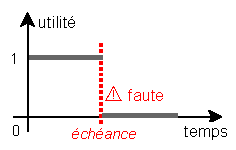
\includegraphics[width=\linewidth]{schemas/SdF_TempsReelDUR}
				\caption[]{Temps-réel dur}
				\label{fig:tempReelDur}
			\end{subfigure}
			\begin{subfigure}{.3\textwidth} \centering
				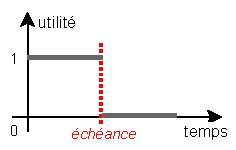
\includegraphics[width=\linewidth]{schemas/SdF_TempsReelFERME}
				\caption[]{Temps-réel ferme}
				\label{fig:tempReelFerme}
			\end{subfigure}
			\begin{subfigure}{.3\textwidth} \centering
				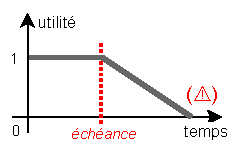
\includegraphics[width=\linewidth]{schemas/SdF_TempsReelMOU}
				\caption[]{Temps-réel mou}
				\label{fig:tempReelMou}
			\end{subfigure}
			\caption{Modèles d'utilité des résultats d'une tâche temps-réel}
			\label{fig:ModelesTempsReel}
		\end{figure}
		
		Plus généralement, les applications embarquées se caractérisent par un ensemble de tâches logicielles qui interagissent entre-elles. Elles sont soit périodiques (c.-à-d. exécutés à intervalle réguliers) soit apériodique (sur réception d'un événement). Chaque tâche possède ses spécifications propres en termes de données d'entrée, de sortie ainsi que ses paramètres d'exécution (selon les cas : période, niveau de priorité, allocation physique) dont une échéance d'exécution. Les systèmes temps-réel peuvent se catégoriser en 3 catégories qui sont schématisées en~\autoref{fig:ModelesTempsReel}. On retrouve d'une part les systèmes \textbf{temps-réel strict} ("\textit{hard real-time}") où le respect de l'échéance est strict en~\autoref{fig:tempReelDur}. Il est alors considéré qu'une tâche dont le temps de réponse dépasserait l'échéance serait une faute temporelle indésirable et les données renvoyées par la tâche n'ont plus de valeur. Le même modèle mais sans conséquences après dépassement de l'échéance est nommé \textbf{temps-réel ferme} ("\textit{firm real-time}") illustré en~\autoref{fig:tempReelFerme}. À l'inverse, les systèmes \textbf{non-temps-réel} n'imposent pas de contraintes d'échéance sur l'exécution des tâches. Il s'agit donc de faire au mieux, mais tout dépassement des temps d'exécution nominaux n'a pas de répercussions. C'est ce que l'on côtoie couramment via nos appareils de tous les jours comme le smartphone ou l'ordinateur. Enfin, les systèmes \textbf{temps-réel souple} ("\textit{soft real-time}") sont un entre-deux où l'échéance représente un seuil limite au-delà duquel la valeur de retour de la tâche garde une utilité pour le système mais qui décroît avec le temps, jusqu'à ne plus être pertinente comme représenté en~\autoref{fig:tempReelMou}. On dit alors que la donnée est "périmée". Ce dépassement peut alors provoquer ou non une faute.
		
		Les analyses d'exécution temporelles des tâches constituent alors un aspect essentiel du développement de logiciel critique afin de garantir le respect des échéances. Cela peut se faire soit de façon expérimentale ou théorique. L'objectif étant de vérifier l'ordonnancement, c'est-à-dire la bonne gestion de l'exécution du logiciel sur le processeur suivant les contraintes imposées (échéances, dates d'activation, périodes...). Un système est dit prédictible si l'on est capable de prouver de façon théorique que les contraintes temporelles seront respectées. Cela se fait par le biais d'analyses d'ordonnançabilité. Un technique classique de ce type d'analyse consiste à évaluer les pires temps d'exécution ("\textit{Worst-Case Execution Time -- WCET}"). Le WCET indique la durée maximum au-delà de laquelle on sait qu'en toutes conditions, la tâche correspondante aura terminé son exécution. Il est possible de comparer les WCET des tâches avec leurs échéances. Pour du temps réel strict, les valeurs de WCET se devront d'être strictement inférieures aux échéances, là où pour du temps réel ferme ou souple on pourra se contenter d'estimation ou de résultats statistiques.
				
		Au sein d'un même processeur, toutes les tâches n'auront potentiellement pas les mêmes types de contraintes d'exécution. Mais en plus de cela, les architectures matérielles multicœurs complexifient d'autant plus l'analyse. 
		
		
	\paragraph{Ressources Partagées}
	
		Comme nous l'avons vu précédemment sur l'architecture multicœur, il existe un bon nombre de ressources qui sont partagées entre les différents logiciels qui sont exécutés. Ces partages de ressources peuvent influencer directement sur l'exécution des tâches et donc sur leur capacité à respecter les échéances. En effet, si plusieurs tâches ont des besoins concurrents d'accès à une même ressource alors nécessairement l'une va passer avant l'autre. Cette dernière sera \textit{de facto} retardée dans son exécution. Il existe ainsi de nombreuses sources de retards potentiels d'exécution~\cite{kotaba_multicore_2013}~: 
		\begin{itemize}
			\item Mémoire --
			\begin{itemize}[label=$ \circ $] %\bigstar \blacklozenge \blacksquare \blacktriangle \blacktriangledown \lozenge \Diamond  \bullet
				\item 	erreurs en lecture~: si une donnée n'est plus présente en cache du fait qu'elle a été remplacée par les données d'une autre application. Cela demande alors à remonter sur les niveaux de mémoire supérieurs, ce qui engendre des temps d'accès supplémentaires importants ;
				\item 	accès concurrents : l'accès concurrent à un niveau de mémoire partagée se fait par le bien d'un contrôleur d'accès mémoire, qui va devoir arbitrer sur l'ordre et le temps alloué à chaque tâche.
				\item 	Cohérence mémoire : selon les technologies de gestion de cache utilisées, il faut gérer la cohérence mémoire. Si une donnée est utilisée dans plusieurs mémoires non partagées, alors il faut s'assurer que la donnée en question reste cohérente entre toutes les tâches qui s'en servent. Cela implique en général une synchronisation sur les niveaux de mémoire supérieure quand elle est modifiée de façon locale, et inversement une propagation des modifications vers les tâches qui manipulent la donnée.
			\end{itemize}
			\item Périphérique et I/O en général --
				chaque périphérique dispose de son propre contrôleur d'accès. On a donc les mêmes enjeux qu'avec les accès concurrents à la mémoire dans le cas où plusieurs tâchent utilisent la même entrée/sortie. Le cas principal ici pour une architecture embarquée est sur l'utilisation d'un bus de communication externe qui sert à interconnecter les calculateurs. L'envoi et la lecture de message sur de tels bus de communication peuvent alors engendrer un grand nombre d'usages concurrents. 
			\item Bus d'interconnexion -- 
				Le fonctionnement même des processeurs implique l'utilisation de bus internes afin de gérer la transmission et le stockage de données. Tout usage de ces bus d'interconnexion peuvent alors impliquer des usages concurrents qui impactent l'accès aux données des tâches.
			\item Puissance de calcul -- 
				Enfin, mais pas des moindres, il n'y aura probablement jamais autant de cœurs que de tâches sur un processeur multicœur. Il est de ce fait évident que les tâches devront se partager tout ou partie des cœurs selon leur allocation physique. C'est là que va entrer en jeu la stratégie d'ordonnancement des tâches. La politique d'ordonnancement joue un rôle essentiel pour permettre le respect des contraintes temporelles et optimiser l'usage de la puissance de calcul pour limiter au maximum les temps d'attente en file d'exécution des tâches. 
		\end{itemize}

\subsection{Problématique et Objectifs}
		Dans le contexte industriel qui concerne notre étude, les évolutions des systèmes cyberphysiques présentés précédemment impliquent que des tâches de différents modèles d'exécution doivent être intégrées au sein d'un même multicœur. On parle alors de système à criticité mixte. Cette coexistence de fonctionnalités va augmenter la complexité d'étude de sûreté de fonctionnement afin de garantir l'ordonnançabilité des tâches et le respect des contraintes temporelles. Et comme nous venons de le voir, les nouveaux calculateurs multicœurs ajoutent en niveau de complexité avec l'augmentation de risque d'interférence entre logiciels concurrents. Il devient par conséquent de plus en plus complexe de mener des études théoriques pour estimer les pires temps d'exécution et donc l'ordonnançabilité des tâches. La conséquence directe à cela est un manque de garanties claires sur le bon respect des échéances temporelles pour les tâches les plus critiques pour lesquelles on ne peut se permettre de telles fautes.
		
		On verra qu'il existe de nombreuses méthodes qui permettent de réduire les interférences et donc fiabiliser les études d'ordonnançabilité. Cependant, cela se fait en général au prix d'un compromis sur les performances de calcul.
		Hors, c'est pour cette même puissance de calcul que la transition vers des calculateurs multicœurs s'est faite. Il semble alors essentiel de vouloir l'exploiter au maximum. On a deux objectifs qui s'opposent, mais qui sont tout autant essentiels. D'une part l'exploitation au maximum des capacités de calcul pour héberger tout le logiciel nécessaire aux nouvelles fonctionnalités des systèmes embarqués. D'autre part continuer à donner des garanties fortes de respect des contraintes temps réel pour les tâches critiques. 
		
		Cela nous mène donc à la problématique centrale de cette thèse, qui est d'identifier les leviers et mécanismes qui peuvent permettre d'atteindre au mieux les deux objectifs susmentionnés d'optimisation de l'usage du processeur avec les garanties temporelles liées aux systèmes critiques. 
		Nous tenterons dans la suite de proposer une réponse à cette problématique par le biais d'une nouvelle approche qui mène à l'usage d'un mécanisme de surveillance et de contrôle de l'exécution des tâches pour éviter toute faute temporelle en cas d'occurrences d'interférences tout en permettant par ailleurs de libérer toute la puissance de calcul disponible dans l'exécution des tâches.
	

\section{Contraintes et Hypothèses}
		
	\subsection{Contexte industriel Automobile}
		Cette problématique s'inscrit dans un contexte industriel aux contraintes spécifiques. Il est donc important d'avoir ces éléments en ligne de compte pour proposer une analyse et des contributions pertinentes. Historiquement dans le domaine automobile, les calculateurs embarqués étaient conçus de manière \emph{ad hoc}. Le logiciel et le matériel étaient intimement liés. Cela conduit à un nombre de calculateurs très important, chaque calculateur apportant une fonctionnalité qui lui est propre. Les architectures se composent alors d'un grand nombre d'unités de calcul interconnectées. 
%		Dans les systèmes automobiles, on peut noter trois principales propriétés dans ces ECU (\textit{Electronic Control Unit})~:
%		\begin{itemize}
%			\item \emph{interconnectés},
%			\item les applications et services sont intégrés dans des sous-systèmes complexes (\emph{Software Components}),
%			\item les fonctions sont \emph{distribuées} sur plusieurs calculateurs.
%		\end{itemize}
		Ce type d'architecture distribuée présente des inconvénients évidents en terme d'évolutivité du système et de coût de développement. À chaque changement de support physique le logiciel doit passer par un nouveau stade de développement plus ou moins conséquent. Inversement, une mise à jour du logiciel ou un ajout de fonctionnalité demande une prise en compte de l'intégration matérielle avec potentiellement des modifications matérielles pour suivre les évolutions. Chaque ajout de fonctionnalités va de cette façon ajouter de nouveaux calculateurs dédiés, complexifiant d'autant plus l'architecture.
		
		Toutes ces contraintes de développement s'inscrivent dans un contexte bien cadré par des normes et standards. L’architecture fédérée telle qu'elle arrive dans les architectures électriques et électroniques abolit la séparation physique qui préexistait entre les composants logiciels, par leur agrégation dans un nombre réduit de calculateurs plus puissants. Cela résulte en un accroissement de la complexité de l’intégration et de la mise en œuvre de la sûreté de fonctionnement. 
	
		\subsection{Standards industriels et Concept de Criticité}	
		Les processus de développement de systèmes embarqués sont régis par des standards qui donnent des garanties sur le bon fonctionnement et donc vis-à-vis du respect des contraintes non fonctionnelles. Ces standards recommandent des directives de développement qui suivent toutes la durée du processus, de la spécification jusqu'aux tests de validation et d'intégration. Une des normes "mères" de la sûreté de fonctionnement des architectures électriques et électroniques est IEC-61508~\cite{iec61508}. Il s'agit d'un standard européen générique qui touche donc à de nombreux domaines tels que le ferroviaire, l'automobile, l'aéronautique, etc. Il s'agit en particulier des systèmes où il existe des risques pour les personnes ou sur l'environnement en cas de défaillances. Ce standard définit des niveaux de criticité SIL (\textit{Safety Integrity Level}). Cela fourni des niveaux de fiabilité requis pour chaque niveau de criticité ainsi que les méthodes applicables pour atteindre cet objectif. Ce standard a été par la suite décliné suivant les domaines. Dans l'automobile est ainsi apparue en 2011 la première version d'ISO 26262, "Véhicules Routiers - Sécurité fonctionnelle~\cite{iso_tc22sc3wg16_iso_2011}. 

		
		La norme ISO 26262 est la norme de référence pour la sûreté de fonctionnement dans le domaine automobile. Elle recommande des méthodes et mécanismes, applicables durant toutes les phases de développement du véhicule, pour atteindre et justifier son niveau de sûreté de fonctionnement. La norme préconise d’effectuer une phase d’analyse des risques pour identifier les situations dangereuses et les classifier en 4 niveaux de criticités nommés ASIL (\textit{Automotive Safety Integrity Level}) allant du moins critique (ASIL A) au plus critique (ASIL D). Pour la détermination de ces niveaux, trois critères sont pris en compte: la sévérité, la probabilité d'accomplissement et la contrôlabilité.
		
		\begin{itemize}
			\item 		\textbf{La Sévérité}	\\
			Les conséquences en cas de défaillance peuvent être Légères et Modérées (\emph{S1}), Sévères et potentiellement mortelles -- mais survie probable -- (\emph{S2}), Potentiellement mortelles -survie incertaine- voire mortelles (\emph{S3}). 		
			\item 		\textbf{La Probabilité} 	\\
			Le risque d'occurence peut être Très Faible (\emph{E1}), Faible (\emph{E2}), de probabilité Moyenne (\emph{E3}) ou de Haute probabilité (\emph{E4}).
			\item 		\textbf{La Contrôlabilité}	\\
			Les capacités de l'utilisateur à gérer la défaillance. Une défaillance peut être facilement contrôlable (\emph{C1}), normalement contrôlable (\emph{C2}), difficilement, voire impossible à contrôler (\emph{C3}).
		\end{itemize}
		
		Bien entendu, l'interprétation de ces trois critères doit se faire au regard du système étudié, et non de façon absolue et déterministe. 
		Ces critères donnent lieu à une table de classification qui définit alors le niveau d'ASIL des composants tel que décrit dans le~\autoref{tab:ASILTable}. On remarquera le niveau "QM" pour \textit{Quality Management}, qui correspond aux composants qui n'impliquent pas de criticité particulière et peuvent alors être développés "au mieux" sans contrainte spécifique. Il est bien entendu moins critique qu'un ASIL A. Avec cette table on connaît alors le niveau de confiance que l'on va imposer à chaque composant pour qu'il puisse être utilisé de façon sûre de fonctionnement. Plus un composant sera critique, plus son niveau d'ASIL sera élevé en conséquence, et donc plus il faudra apporter d'efforts pour qu'il respecte les standards.
		
		\newcommand{\red}{\ccolor{red}} \newcommand{\oran}{\ccolor{orange}} 
		\newcommand{\yel}{\ccolor{yellow}} \newcommand{\gr}{\ccolor{Green}}
		\newcommand{\mc}{\multicolumn} \newcommand{\mr}{\multirow{-4}{*}}
		\begin{table}[ht]
			\centering
			\caption{Matrice de Définition des Niveaux d’ASIL - ISO 26262}
			\label{tab:ASILTable}
			\begin{tabular}{@{}ccccccccccccc@{}}
				\toprule
				 &           & \mc{11}{c}{Contrôlabilité}  \\
				\cmidrule{3-13}
							&           & \mc{3}{c}{\cellcolor{Green}{C1}} & \phantom{} & \mc{3}{c}{\cellcolor{yellow}{C2}} & \phantom{} & \mc{3}{c}{\cellcolor{orange}{C3}}  \\
					\cmidrule{2-2}			\cmidrule{3-5}									\cmidrule{7-9} 									\cmidrule{11-13}
					\mc{2}{r}{Sévérité}  & \gr{ S1 } & \yel{ S2 } & \oran{ S3 } &          & \gr{ S1 } & \yel{ S2 } & \oran{ S3 } &			  & \gr{ S1 } & \yel{ S2 } & \oran{ S3 } \\
				\midrule
				 			&  \gr{ E1 }  &    QM   &     QM     &    QM      &            &    QM    &     QM     &     QM      &			  &    QM     &     QM     &   \gr{ A }  \\
				 			& \yel{ E2 }  &    QM   &     QM     &    QM      &            &    QM    &     QM     &  \gr{ A }   & 			  &    QM     &  \gr{ A }  &  \yel{ B }  \\
				 			& \oran{ E3 } &    QM   &     QM     & \gr{ A }   &            &    QM    &  \gr{ A }  &  \yel{ B }  &			  & \gr{ A }  & \yel{ B }  & \oran{ C }  \\
		   \mr{Probabilité} & \red{ E4 }  &    QM   &  \gr{ A }  & \oran{ B } &            & \gr{ A } & \oran{ B } & \oran{ C }  & 			  & \yel{ B } & \oran{ C } &  \red{ D }  \\
				\bottomrule
			\end{tabular}
		\end{table}

		On peut mentionner de la même manière d'autres standards équivalents dans l'avionique, DO-176 où les niveaux de criticité sont désigné en DAL ("\textit{Design Assurance Level}"), ou encore le ferroviaire avec CENELEC 5012x, mais aussi dans le nucléaire, le spatial, l'automatique, le médical... La plupart dérivés de IEC-61508.  Un certain nombre de ces standards ont été comparés dans les travaux de~\cite{baufreton_multi-domain_2010}. On y retrouve un point commun qui nous intéresse tout particulièrement ici qui est sur les contraintes temporelles.
		
		Que ce soit IEC-61508 ou plus spécifiquement ISO 26262, il est clairement stipulé que 
		"\textit{les contraintes temporelles des fonctions à durée critique doivent être gérées par les spécifications de sûreté de fonctionnement logicielle. Ici, à la fois les pires temps d'exécution au niveau du code et les temps de réponse au niveau système doivent être considérés.}". Et précisément, "\textit{l'absence de tout interférence se doit d'être assuré et, tout comme dans IEC-61508, le logiciel est sujet au plus haut niveau d'ASIL impliqué quand l'indépendance temporelle entre les fonctionnalités ne peut être assurée.}"~\cite{iso_26262-7_road_2018}. C'est au regard de ce type de contrainte industrielle qu'il est essentiel de proposer de nouvelles solutions avec l'arrivée de calculateurs multicœurs qui complexifient grandement les garanties de non-interférence.
	
	\subsection{Contraintes d'intégration}
			
	De façon plus générale, les enjeux industriels peuvent varier selon les domaines. Ceci étant dit on peut nommer des points principaux, qui sont ceux que l'on va tenter de prendre en considération dans cette étude. La première d'entre elle est l'imposition de capacités de déploiement rapides ("\textit{Time-to-market}" réduit). Les itérations entre générations demandent des coûts de développement les moins importants possibles. Cela permet des cycles courts et réactifs qui s'adaptent aux évolutions technologiques. Cette contrainte industrielle est structurante sur les choix de conception, ce qui nous ramène souvent au principe "\emph{KISS}" pour "\emph{Keep It Safe and Simple}" dans notre cas. C'est une philosophie que j'ai souhaité maintenir au long de cette thèse afin de tenter une approche un peu différente des principales recherches actuelles qui tentent souvent d'aller dans des niveaux de détails toujours plus précis et complexes pour répondre aux difficultés technologiques, au détriment d'une facilité d'implémentation qui permettrait une appropriation industrielle. Comme on le verra plus tard, il existe ainsi des solutions très sophistiquées qui donnent de bons résultats théoriques, mais qui ne se sont pas généralisés. Les questions de complexité d'implémentation et simplicité de maintenance dans un cas réel semblent donc relativement déterminantes pour mesurer la pertinence d'une nouvelle contribution à la sûreté des systèmes embarqués. 
	
	En ce sens, il existe globalement 3 types de sous-systèmes qui sont intégrés par les constructeurs. 
	D'abord les systèmes en \textit{black box} ou "boites noires" qui sont entièrement conçu par un équipementier tiers à partir de spécifications. Le contenu de ces "boites" est alors inconnu dans ses détails.
	Ensuite les systèmes en \textit{white box} où à l'inverse, la totalité de sa conception et de son modèle est connu. Cela permet des tests bien plus en profondeur et donc une plus grande confiance en son comportement. Pour être des "boites blanches" les composants sont en général soit directement faits par l'intégrateur final, soit fourni en open-source (plus rare, tristement).
	Enfin, il y a tout l'entre-deux de composants contenants à la fois des éléments en "boite noire" et en "boite blanche", que l'on appelle naturellement "boites grises".
	Il est très important de noter par ailleurs une catégorie transverse des systèmes \textit{"legacy"}, qui sont des composants où les altérations et modifications sont impossibles pour diverses raisons. Soit parce qu'il s'agit d'une black box que l'on ne souhaite ou ne peut remplacer, soit pour des raisons de compatibilité restreinte où toute modification risquerait de compromettre la totalité du système intégré. 
	Ces différents types de sous-systèmes sont importants à présenter, car tout ce qui va toucher aux boites noires et aux composants legacy ajoutent une contrainte forte sur le développement de solutions à la sûreté de fonctionnement. De fait, tout mécanisme de sûreté de fonctionnement impliquant la modification ou l'adaptation du code de fonctions intégrées au système risque d'être éliminé d'office !
	
	On pourra pour finir, mentionner des enjeux plus divers tel que les contraintes d'encombrement. Les systèmes embarqués ont une forte tendance à la miniaturisation pour des raisons diverses selon les domaines. Cela permet une réduction de poids, essentiel pour tous les systèmes volants (avions, drones...) mais aussi d'encombrement pour des domaines comme l'automobile ou le ferroviaire qui doivent en toute circonstance rester dans des dimensions standards. Cette contrainte se fait beaucoup sentir avec l'arrivée des voitures autonomes par exemple, où les premiers prototypes --~bien que fonctionnels~-- se sont avérés trop chargés et encombrants avec le surplus d'équipement pour être transposables facilement en produits commercialisables tel-quel.
	
	Au regard de ces enjeux, l'évolution future naturelle est de réduire le nombre de calculateurs embarqués, en passant d'un grand nombre d'unités de calcul à une quantité limitée de "supercalculateurs", qui vont agréger différentes tâches. On passe de cette façon d'un système distribué à un système fédéré basé sur des calculateurs primaires accompagnés de processeurs satellites qui gèrent le strict nécessaire à hauteur des différents capteurs/actionneurs.  Cela permet de réduire les coûts et l'encombrement, qui va diminuer par la même occasion la quantité de câblages requis. Ce type d'architecture va faciliter l'évolutivité qui sera donc bien plus axée sur des mises à jour logicielles sans toucher au matériel. La connectivité permet de mettre en œuvre le concept du véhicule \textit{"as-a-service"}, qui va pouvoir évoluer et se mettre à jour régulièrement à distance (\textit{Over-the-Air Updates}). 
	
	
\section{Grandes approches du domaine}

	Nous verrons plus en détail dans le~\autoref{chap:2_StateofArt} les différentes solutions actuelles qu'il existe dans le domaine pour répondre à ces problématiques. Nous pouvons tout de même d'ores-et-déjà présenter fondamentalement sur quoi reposent les principes existants afin de mieux situer notre axe de recherche.
	
	La problématique principale à laquelle nous devons faire face réside dans la gestion des interférences matérielles de façon à éviter des fautes temporelles ou tout du moins à couper la chaîne de causalité de façon à ce qu'il y ait toujours silence sur défaillance et donc que le système puisse continuer à fonctionner correctement. Il est possible de différencier deux grands domaines d'approches. D'une part les stratégies de \textbf{contrôle} qui sont plutôt statiques et définis hors-ligne lors du développement ; d'autre part les stratégies \textbf{réactives} qui sont plutôt dynamiques et évoluent en ligne pendant le fonctionnement.
	
	\subsection{Mécanismes de contrôle}
		Ce genre de stratégies consistent à déployer des mécanismes qui limitent les interférences et donc les risques de faute de façon préventive. Le développement et l'implémentation sont alors réalisés d'une manière à ce que par construction, les risquent soit \textit{de facto} rendus impossibles.
		Ce type de stratégies permet de limiter plus efficacement les explosions de pire temps d'exécution notamment, et donc conserver une exécution du logiciel bien cadrée et maîtrisée pour en contrôler les risques inhérents au matériel. 
		
		On peut citer parmi ce genre de techniques : 
		\begin{itemize}
		\item 			Politiques strictes de gestion d'accès aux ressources partagée, avec des intervalles de temps fixes dédiées notamment. Chaque application ayant sa fenêtre temporelle dédiée pour accéder à la ressource partagée, les délais deviennent connus et maîtrisés.
		\item 			Séparation temporelle d'exécution des applications~: il est possible d'ordonnancer les différentes applications de façon complètement séparées les unes des autres. Cela revient à limiter fortement l'exécution parallèle de code, mais par la même prévient radicalement tout risque d'interférence avec le logiciel ainsi isolé.
		\item 			Séparation spatiale des applications~: l'allocation d'un espace mémoire dédié pour chaque application permet de réserver et donc séparer physiquement les applications entre-elles. De cette façon, tout risque de recouvrement des données (c.f. erreurs de lecture) est empêché entre applications qui ont des réservations d'espace mémoire disjoint.
		\end{itemize}
		
		La plupart des méthodes qui rentrent dans cette catégorie ont en revanche un défaut commun qui est de limiter les capacités d'utilisation du matériel. En effet, on comprend naturellement que si l'on limite la taille mémoire qu'une application donnée est autorisée à utiliser pour son fonctionnement, ou encore si l'on contraint sa plage temporelle d'accès à certaines ressources alors les performances de l'ensemble seront forcément moindre que s'il n'y avait pas ces limitations. Des garanties réduites sur les pires temps d'exécution se font donc au détriment de l'optimisation d'utilisation des ressources matérielles. 
		
		Si l'on souhaitait se passer de tels mécanismes en conservant les mêmes niveaux de certitudes sur les durées d'exécution des tâches, cela impliquerait un surdimensionnement non négligeable des processeurs utilisés. 

	\subsection{Mécanismes Réactifs}
		À l'inverse, les stratégies réactives se basent sur l'observation de l'état du système pendant son fonctionnement de façon à agir en conséquence uniquement si nécessaire. Le principe est de monitorer en temps-réel l'exécution des processus et activer sur demande des mécanismes de prévention des fautes. Ce type de méthode est plus complexe à mettre en place et présentent a priori des garanties plus faibles. Cela en fait une solution plus adaptée pour du temps-réel souple tout en conservant des performances moyennes convenables. 
		
		Les systèmes de \textbf{watchdog} sont à la base de ce genre de mécanisme, en levant un traitement d'erreur en cas de constat d'une défaillance, de façon à isoler cette dernière. Cela ne permet pas d'empêcher l'erreur, uniquement de prévenir ou au moins mitiger  toute conséquence supplémentaire.
		
		Les techniques d'ordonnancement dynamique des tâches permettent aussi en un sens d'optimiser l'utilisation des ressources de calcul en priorisant l'exécution au plus urgent par exemple. C'est le cas par exemple d'un ordonnancement des tâches en EDF - "\textit{Earliest Deadline First}", autrement dit "Priorité à l'Échéance au plus Tôt" qui exécute, comme son nom l'indique, systématiquement la tâche dont l'échéance est la plus proche. De façon générale, tout mécanisme de changement dynamique de priorité selon l'état du système entre dans cette catégorie.
		
		Enfin, les mécanismes de réaction consistent essentiellement à suspendre toute tâche indésirable de façon à isoler les tâches temps-réel en cours d'exécution. Par conséquent, cela prévient pendant l'exécution les risques d'interférences matérielles, au détriment temporaire des tâches non critiques. Cela n'est bien entendu possible que dans un cadre où l'on peut modifier en fonctionnement l'exécution des tâches et se permettre d'en stopper une partie. Certains mécanismes réactifs sont à usage unique dans le sens où une fois ce déclenchement fait, le système reste dans un fonctionnement en mode dégradé pour tout le reste de son exécution. À l'inverse d'autres solutions proposent un mode dégradé temporaire avec un retour en fonctionnement nominal une fois le risque passé. 
		
		La plus grande difficulté de ces stratégies réside donc dans la preuve des garanties qu'elles sont capables de fournir sur les propriétés de sûreté de fonctionnement au regard des exigences non fonctionnelles définies. Elles permettent de mieux exploiter les ressources disponibles. Les systèmes réactifs sont par exemple à la base des usages informatiques grand public qui reposent sur un système d'exploitation standard pour lesquels il n'y a pas de contrainte temporelle dure.


\section{Contribution de la thèse et objectifs}

	Dans le cadre de l'utilisation de calculateurs multicœurs dans les applications industrielles, nous aborderont dans cette thèse les difficultés que cela implique en terme d'implémentation pour continuer à garantir le bon fonctionnement du logiciel. Plus spécifiquement, nous nous intéresseront aux implications du partage de ressources sur les temps d'exécution de logiciel critiques dans le cadre de systèmes à criticité mixte. Ces partages pouvant entraîner des congestions qui en conséquence ajoutent des latences qui peuvent aller jusqu'à provoquer des dépassements d'échéance temporelle et donc des fautes logicielles temporelles transitoires. Pour empêcher ce risque potentiellement critique, il sera proposé un mécanisme novateur de Surveillance et de Contrôle d'exécution logiciel. Les objectifs ici sont multiples, car d'une part, l'on souhaite conserver des garanties sur les temps d'exécution de logiciel critique, mais en même temps il faut trouver des mécanismes les moins intrusifs possibles sur l'exécution pour profiter au maximum des puissances de calcul multicœur mis à disposition. 
	
	Pour cela, nous verrons dans le~\autoref{chap:2_StateofArt} sur l'État de l'Art les différents propositions existantes qui permettent de répondre à tout ou partie des objectifs susmentionnés. %\alert{[Détailler sur le contenu état de l'art]}.
	
	Par la suite le~\autoref{chap:3_PrincipeArchi} présentera notre façon d'aborder la question avec nos hypothèses et modélisation du système. Dans le cadre d'un système multicœur qui héberge des applications à criticité mixte, on verra le modèle d'exécution adopté, orienté vers une approche originale basé sur des chaînes de tâches. Cela va impliquer des notions de précédence d'exécution et de temps de réponse bout-à-bout qui seront essentiels par la suite.
	
	Cela nous mènera dans le~\autoref{chap:4_ProtocolExpe} suivant à développer notre mécanisme de Surveillance et Contrôle basé sur ces chaînes, son architecture et ce que cela implique en terme d'implémentation. Cette approche se basera sur la surveillance des contraintes temporelles de chaînes de tâches dans un système à criticité duale, exécuté sur un multicœur bien entendu. L'objectif étant de stopper temporairement des tâches non critiques pour éviter des interférences qui risqueraient de provoquer des fautes temporelles.
	
	Enfin, nous verrons en~\autoref{chap:5_ImplementationCase} un cas d'implémentation qui a pu être réalisé sur une plateforme d'essai. Cette plateforme se voulant être une preuve de concept, l'objectif est de voir l'influence et les tenants et aboutissants du mécanisme proposé. Nous utiliserons pour cela des tâches d'une suite de benchmark sur laquelle on pourra implémenter le mécanisme, le calibrer et en tirer des mesures de performance.
	
	En conclusion, nous ferons un bilan des résultats obtenus avec des perspectives d'utilisation, ainsi que des pistes de recherche. 
    
%% transition - présentation contenu État de l'Art %%


\ifdefined\included
\else
\bibliographystyle{StyleThese}
\bibliography{these}
\end{document}
\fi
